\section{Experiments}

\subsection{Experimental Questions}

\begin{itemize}[leftmargin=*]
  \item Q1: Under low-quality replay data, do policy/behavior regularization methods outperform a weak TD3+BC anchor?
  \item Q2: Is SSAR's gain plausibly tied to trusted-action selection rather than generic regularization?
  \item Q3: Can ATLAS distill the trusted-action signal into a reusable selector?
  \item Q4: Does the offline advantage persist during online fine-tuning?
  \item Q5: If fixed teacher regularization hurts online adaptation, does a simple release schedule recover the loss?
\end{itemize}

\todobox{A-line owner: add the value-conservatism experimental question after CQL / Cal-QL results arrive.}
\todobox{B-line owner: add the non-conservative online contrast question after PPO / SAC / vanilla results arrive.}

\subsection{Main Offline and Mechanism Results}

Environment: \texttt{hopper-medium-replay-v2}.

\begin{table}[t]
\centering
\scriptsize
\setlength{\tabcolsep}{2.5pt}
\begin{tabular}{@{}lrrrrrl@{}}
\toprule
Method & Seed & Steps & Eval eps & Final & Best & Interpretation \\
\midrule
TD3+BC & 0 & 50k & 5 & 22.43 & 22.43 & weak anchor \\
ReBRAC-lite & 0 & 50k & 5 & 34.48 & 34.48 & stronger regularized baseline \\
PRDC official & 0 & 50k & 5 & 23.54 & 23.54 & no clear uplift in smoke \\
A2PR official & 0 & 50k & 5 & 22.31 & 22.81 & no clear uplift in smoke \\
SSAR full IQL-qv & 0 & 50k & 5 & 38.56 & 43.97 & strongest 50k modern baseline \\
SSAR cached IQL-qv & 0 & 100k & 5 & 92.44 & 100.98 & high-variance upper anchor \\
SSAR full IQL-qv & 1 & 100k & 20 & 60.88 & 99.22 & near-100 spike repeats; unstable final \\
IQL compact & 0 & 100k & 5 & 45.27 & 81.28 & strong value-style baseline \\
CQL compact & 0 & 50k & 5 & 39.81 & 39.81 & conservative value anchor \\
ATLAS & 0 & 100k & 5 & 69.97 & 69.97 & positive offline signal \\
ATLAS & 1 & 100k & 20 & 68.11 & 68.11 & seed stability check \\
ATLAS shuffled labels & 0 & 50k & 5 & 18.78 & 19.35 & label alignment matters \\
\bottomrule
\end{tabular}
\caption{C-line offline and mechanism results on \texttt{hopper-medium-replay-v2}.}
\label{tab:c-main}
\end{table}

\begin{figure}[t]
\centering
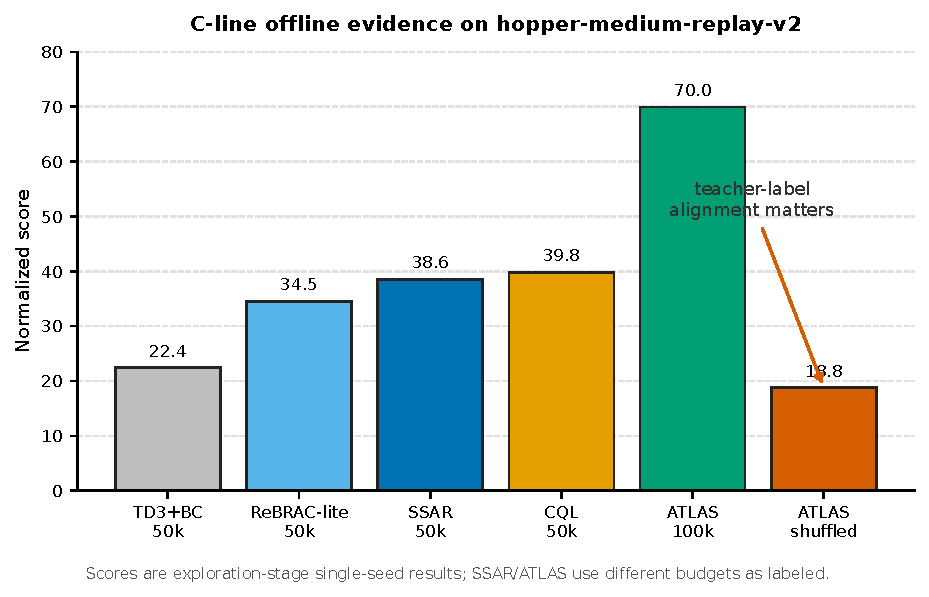
\includegraphics[width=0.92\linewidth]{../figures/fig3_offline_results.pdf}
\caption{C-line offline evidence on \texttt{hopper-medium-replay-v2}. Aligned ATLAS labels improve the offline endpoint, while shuffled labels collapse.}
\label{fig:offline-results}
\end{figure}

\subsection{Second Replay Environment}

\begin{table}[t]
\centering
\small
\begin{tabular}{lrrrrrl}
\toprule
Method & Seed & Steps & Eval eps & Final & Best & Interpretation \\
\midrule
SSAR full IQL-qv & 0 & 100k & 10 & 94.28 & 94.60 & strong teacher anchor \\
ATLAS & 0 & 100k & 10 & 71.26 & 77.86 & signal survives, but gap remains \\
\bottomrule
\end{tabular}
\caption{Second-environment check on \texttt{walker2d-medium-replay-v2}.}
\label{tab:walker}
\end{table}

\subsection{P0 Offline-to-Online Eval20 Panel}

Environment: \texttt{hopper-medium-replay-v2}, seed0, 50k offline + 10k online, 20 evaluation episodes. This panel is the current P0 evidence for whether trusted-action offline gains survive online fine-tuning.

\begin{table}[t]
\centering
\scriptsize
\resizebox{\textwidth}{!}{%
\begin{tabular}{lrrrrrl}
\toprule
Method & Offline final & Offline best & Online final & Online best & Best step & Interpretation \\
\midrule
TD3+BC release & 22.20 & 22.20 & 40.06 & 40.06 & 60k & weak offline anchor, best final online score \\
TD3+BC fixed & 22.20 & 22.20 & 33.35 & 46.12 & 58k & improves online, less stable tail \\
ATLAS release & 46.70 & 46.70 & 37.50 & 38.79 & 56k & strong offline endpoint, lower online final \\
ATLAS fixed & 46.70 & 46.70 & 28.93 & 32.80 & 53k & fixed teacher constraint hurts most \\
Random trust release & 12.14 & 19.95 & 35.53 & 44.13 & 57k & matched trust fraction without alignment fails offline \\
SSAR/IQL-qv release & 50.71 & 50.71 & 28.87 & 31.85 & 58k & strongest offline endpoint, worst online final \\
SSAR/IQL-qv fixed & 50.71 & 50.71 & 38.61 & 96.22 & 57k & large transient spike, tail drops below TD3+BC release \\
\bottomrule
\end{tabular}
}
\caption{Required P0 offline-to-online eval20 panel. ``Release'' means the offline BC/teacher coefficient is linearly decayed during online fine-tuning; ``fixed'' keeps it constant.}
\label{tab:o2o}
\end{table}

\begin{figure}[t]
\centering
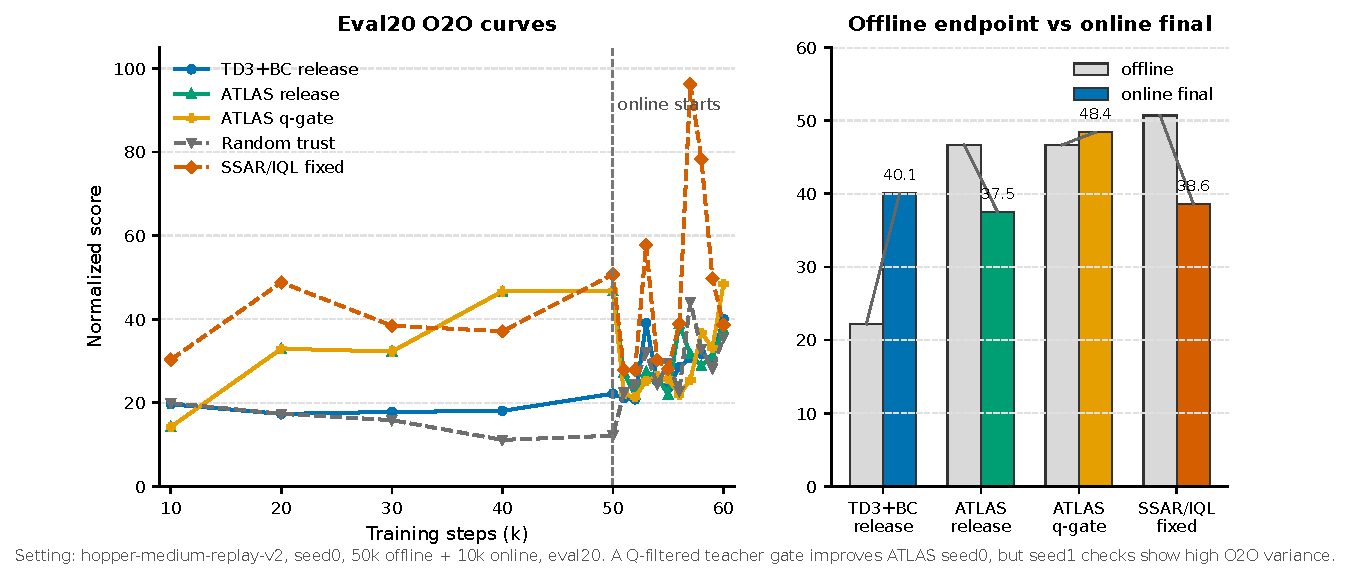
\includegraphics[width=0.92\linewidth]{../figures/fig4_o2o_curve.pdf}
\caption{P0 offline-to-online eval20 panel. Stronger teacher labels improve offline endpoints but do not improve final online score under the current online regularizer.}
\label{fig:o2o-curve}
\end{figure}

The random-subset control is important: it preserves the IQL-qv hard-trust fraction but breaks transition-label alignment, and it loses the offline benefit. The online panel therefore does not say that trusted labels are useless. It says that aligned trusted labels help offline learning, but the same teacher constraint is not a sufficient online adaptation mechanism in this runner.

\todobox{C-line owner: if one more C-line run is launched, prioritize a better online adaptation mechanism for teacher labels, not PRDC/A2PR expansion.}

\subsection{Q-Filtered Trust Diagnostic}

Gemini-based external review identified the main weakness of Table~\ref{tab:o2o}: the release schedule diagnoses over-constraint but does not fix it. We therefore add a minimal online gate that keeps teacher BC regularization only when the current critic rates the dataset action above the current policy action.

\begin{table}[t]
\centering
\scriptsize
\resizebox{\textwidth}{!}{%
\begin{tabular}{llrrrrrl}
\toprule
Seed & Method & Offline final & Offline best & Online final & Online best & Best step & Interpretation \\
\midrule
0 & ATLAS fixed & 46.70 & 46.70 & 28.93 & 32.80 & 53k & fixed teacher constraint traps adaptation \\
0 & ATLAS Q-gate fixed & 46.70 & 46.70 & 48.41 & 48.41 & 60k & seed0 positive: gate repairs final score \\
0 & SSAR/IQL Q-gate fixed & 50.71 & 50.71 & 38.88 & 65.73 & 57k & reduces collapse vs release, but still unstable \\
1 & TD3+BC release & 20.19 & 20.96 & 98.86 & 98.86 & 60k & seed1 shows very high O2O variance \\
1 & ATLAS release & 31.21 & 31.21 & 84.35 & 84.35 & 60k & release helps seed1, but below TD3+BC \\
1 & ATLAS fixed & 31.21 & 31.21 & 23.88 & 49.92 & 57k & fixed constraint still poor \\
1 & ATLAS Q-gate fixed & 31.21 & 31.21 & 39.91 & 70.03 & 56k & improves over fixed, below release and TD3+BC \\
\bottomrule
\end{tabular}
}
\caption{Q-filtered trust diagnostic. Q-gating is promising on seed0, but seed1 prevents a stable superiority claim.}
\label{tab:qgate}
\end{table}

The diagnostic changes the story but does not finish it. Q-gating is the first mechanism that makes ATLAS beat TD3+BC on seed0 final score. However, seed1 shows that TD3+BC can itself jump to near-expert performance in this short Hopper O2O slice, while ATLAS release reaches 84.35 and Q-gated fixed reaches 39.91. We therefore treat Q-filtered trust as the next method hypothesis, not as a solved contribution.

\subsection{Cross-Line Fill-In Table}

\begin{table}[t]
\centering
\small
\resizebox{\textwidth}{!}{%
\begin{tabular}{llllllllrrl}
\toprule
Track & Family & Method & Env & Seed & Offline & Online & Eval eps & Final & Best & Status \\
\midrule
A & Value conservatism & TODO & hopper-medium-replay-v2 & 0 & TODO & TODO & TODO & TODO & TODO & waiting \\
B & Non-conservative contrast & TODO & hopper-medium-replay-v2 & 0 & TODO & TODO & TODO & TODO & TODO & waiting \\
C & Policy regularization & TD3+BC O2O release & hopper-medium-replay-v2 & 0 & 50k & 10k & 20 & 40.06 & 40.06 & done \\
C & Trusted-action selection & ATLAS O2O release & hopper-medium-replay-v2 & 0 & 50k & 10k & 20 & 37.50 & 38.79 & done \\
C & Trusted-action selection & SSAR/IQL-qv O2O fixed & hopper-medium-replay-v2 & 0 & 50k & 10k & 20 & 38.61 & 96.22 & done \\
C & Trusted-action selection & ATLAS offline & hopper-medium-replay-v2 & 0 & 100k & 0 & 5 & 69.97 & 69.97 & done \\
C & Trusted-action selection & ATLAS offline & hopper-medium-replay-v2 & 1 & 100k & 0 & 20 & 68.11 & 68.11 & done \\
\bottomrule
\end{tabular}
}
\caption{Template table for merging A/B/C-line results.}
\label{tab:cross-line}
\end{table}

\todobox{A-line owner: replace the A row with real method, steps, eval episodes, final/best score, and log path.}
\todobox{B-line owner: replace the B row with real method, steps, eval episodes, final/best score, and log path.}
